\section{实验目的}
本次实验有以下五个实验目的:
\begin{enumerate}
    \item 理解CPU Cacheline、流水线冒险(hazard)及相关性,在Lab05的基础上设计简单流水线CPU
    \item 在1.的基础上设计支持Stall的流水线CPU。通过检测竞争并插入停顿(Stall)机制来解决数据冒险、控制冒险和结构冒险。
    \item 在2.的基础上,增加Forwarding机制来解决数据竞争,减少因数据竞争带来的流水线停顿时,提高流水线处理器的性能。
    \item 在3.的基础上,通过predict-not-taken策略解决控制冒险,减少控制竞争带来的流水线停顿时,进一步提高处理器性能。
    \item 在4.的基础上,将CPU支持的指令由16条扩充至31条,使处理器功能更加丰富。
\end{enumerate}

\section{原理分析}
\subsection{流水线(Pipeline)的原理}
MIPS的CPU包含了五级流水,分别是取指令阶段(IF)、译码阶段(ID)、执行阶段(EX)、访存阶段(MA)、写回阶段(WB)。流水线示意图如图\ref{fig:pipeline},本图来自Lab06实验指导书。接下来将详细介绍每个阶段的功能。
\begin{figure}[!h]
    \centering
    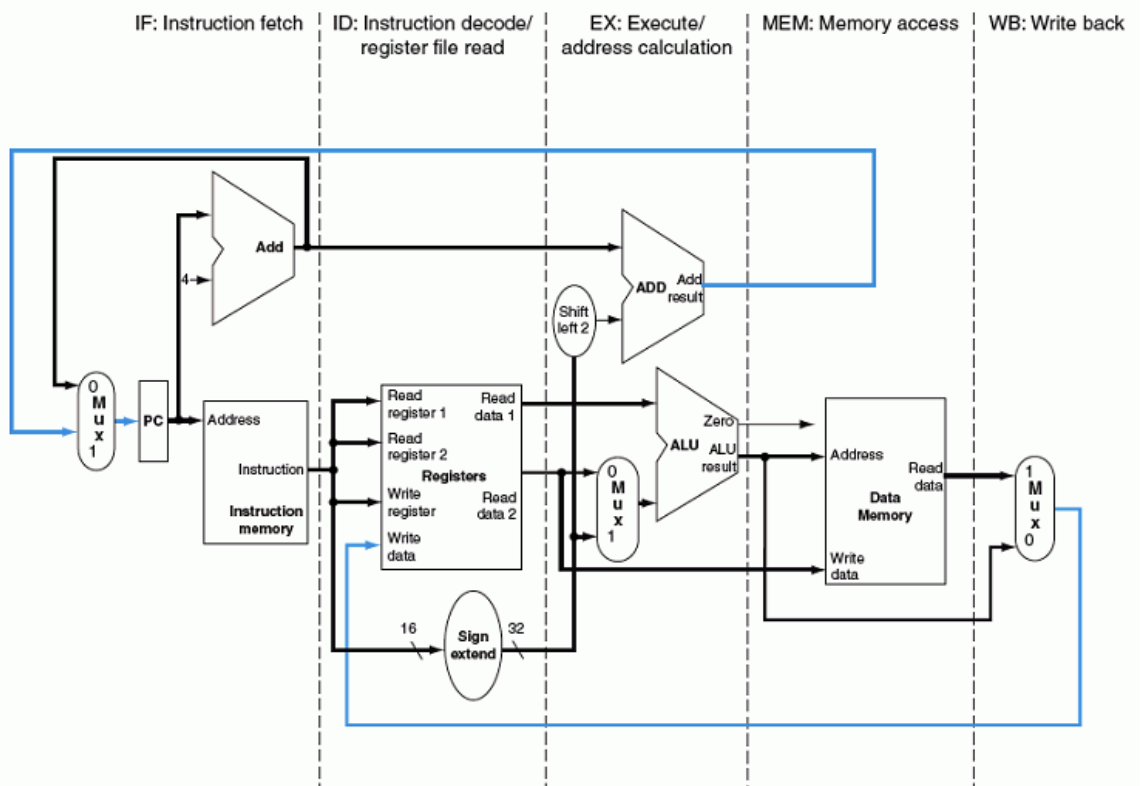
\includegraphics[width=0.7\textwidth]{./pipeline.png}
    \caption{流水线示意图}
    \label{fig:pipeline}
\end{figure}

\subsubsection{取指令阶段(IF)}
在取指令阶段,CPU会根据PC给出的地址,访问指令存储器,取出所对应的指令,并存放在IF/ID段寄存器中。除此以外还需要计算PC+4的值以更新PC的值。

\subsubsection{译码阶段(ID)}
在译码阶段,涉及到的子模块主要包括主控制器模块 (Ctr)、寄存器模块 (Register)、符号扩展模块。在这一阶段主要的功能有:主控制器(Ctr)产生控制信号,寄存器模块(Registers)读取寄存器数据,符号扩展模块(Sign Extension)将16位立即数扩展为32位。除此以外,根据IF/ID段寄存器中的指令,选择rt或者rs寄存器进行访问,并将指令解析从而决定是否需要进行写入操作。
\textbf{需要特别注意的是}此阶段仅选择出写入寄存器,并不会实际执行写操作,选择结果会一直保存到写回阶段(WB)阶段才进行实际写入。

为了进一步提高流水线的效率,对于无条件跳转指令 j、jal、jr,其对应的所有操作都会在本阶段完成。

\subsubsection{执行阶段(EX)}
执行阶段,顾名思义,就是指令开始运行的阶段,涉及的子模块基本全是围绕ALU展开的,如ALU控制单元(ALUCtr),ALU单元以及与之相关的多路选择器(Mux)。其主要功能是ALU会根据ALUCtr的输出AluCtrOut来对输入进行相应的算数运算。
对于 beq、bne 指令,本阶段也会决定是否需要跳转。
对于lui指令,lui所对应的多路选择器会选取指令中立即数部分作为本阶段的执行结果的高16位,因此需要舍弃此时ALU的输出。
\textbf{注:}因为我在本实验中将指令拓展为了31条,而新增加的指令包含了bne和lui,所以需要做此说明。具体的扩展将在之后展开。

\subsubsection{访存阶段(MA)}
在访存阶段,主要进行内存模块的访问,主要涉及内存模块。
如果该指令需要内存访问,则需要向数据存储器(Data Memory)提供地址,并保存数据存储
器的输出。如果该指令为跳转指令 (beq、jr、jal 等),则需要将跳转目标地址写入PC,
并且刷新流水线。

\subsubsection{写回阶段(WB)}
写回阶段主要包括寄存器模块。在执行前需要确定是否需要向寄存器写入以及写入的数据是ALU的运算结果还是访问内存得到的数据,但无论如何写入的数据一定会在访存阶段(MA)确定下来。
除此以外,正如2.1.2节所描述的,写入寄存器的编号在译码阶段(ID)阶段也已经确定。

\subsection{主控制器(Ctr)的原理}

主控制单元根据输入指令的$[31 :26]$位的opCode,将指令分成R型(add,sub,and,or,slt)、I型(lw,sw,beq)和J型(j,jal),
并且输出相对应的信号至regDst、aluSrc、memToReg、regWrite、memRead、memWrite、branch、aluOp和jump。考虑到此次支持的指令中包含了立即数运算,且andi和ori需要零扩展,所以还需要增加一个信号extSign来表示当前是否需要有符号扩展。指令中还包含了jal,与j指令类似,也需要设置一个jalSign来表示当前指令是否是jal。

除此以外,在2.1.2节提到,为了提高流水线的效率,无条件跳转指令jr的所有操作必须在译码阶段(ID)完成,而之前的jrSign是由在执行阶段(EX)才会使用的ALUCtr产生的。为了解决这个问题,我修改了主控制器的输出,使之能够输出jrSign。因为本处理器支持31条指令,所以还添加了条件跳转指令的信号beqSign和bnqSign,原来的条件跳转指令branch就无需存在了。对于需要舍弃ALU输出的lui指令,也需要专门的信号来表示,因此还添加了luiSign。

根据理论课程知识可以得到输出信号的作用如下表\ref{1}。

\begin{table}[H]
    \centering
    \begin{tabular}{c|p{12cm}}
    \hline
        信号&作用  \\
        \hline
        regDst &目标寄存器的选择信号,若为0则写入rt代表的寄存器,为1则写入rd代表的寄存器 \\
        aluSrc & 取值为0表示使用rt作为输入,取值为1表示使用立即数作为输入\\
        memToReg & 取值为0表示使用ALU的输出作为写寄存器的输入数据,取值为1表示从内存中读取数据\\
        regWrite & 取值为1表示当前指令需要执行寄存器写入操作\\
        memRead & 取值为1表示当前指令需要从内存中读取数据(load)\\
        memWrite & 取值为1表示当前指令需要将数据写入内存(store)\\
        aluOp[2:0] & 输出至AluCrtr来进一步确定信号类型,将在下表中详细展开\\
        jump & 取值为1表示当前指令为无条件跳转指令(jump)\\
        jalSign & 取值为1表示当前指令为jal指令(jal)\\
        extSign & 取值为1表示当前指令需要有符号扩展\\
        luiSign & 取值为1表示当前指令为lui指令(lui)\\
        beqSign & 取值为1表示当前指令为beq指令(beq)\\
        bneSign & 取值为1表示当前指令为bne指令(bne)\\
        jrSign & 取值为1表示当前指令为jr指令(jr)\\
        \hline
    \end{tabular}
    \caption{主控制单元输出信号的作用}
    \label{1}
\end{table}

因为aluOp所需分辨的指令超过4条,无法继续使用2位二进制数来表示,因此aluOp需要3位二进制数来保存。不同的二进制位的组合对应了不同的指令操作。但是在该指令实际运行之前,其还必须被输出至AluCtr,最后才能被Alu模块所执行。
在本实验中,aluOp与MIPS自身的aluOp使用习惯保持一致,以减小之后出现差错的可能性。此处和Lab05保持一致,对应关系如表\ref{3}。

\begin{table}[H]
    \centering
    \begin{tabular}{c|c|c}
    \hline
        aluOp& 指令 & 具体操作\\
        \hline
        000 & lw,sw,addi,addiu &ALU进行加法操作\\
        001 &beq&ALU进行减法操作\\
        010 & slti&ALU进行有符号的比较\\
        011 & andi&ALU进行逻辑与操作\\
        100 & ori&ALU进行逻辑或操作\\
        101 & R&结合Funct域的六位进行判断\\
        110 & sltiu&ALU进行无符号的比较\\
        111 & xori&ALU进行逻辑异或\\
        \hline
        
    \end{tabular}
    \caption{aluOp与输出信号之间的对应关系}
    \label{3}
\end{table}

结合实验指导书,可以得出以下的opCode与输出信号之间的对应关系,如表\ref{4},\ref{5}。

\begin{table}[H]
    \centering
    \begin{tabular}{c|c|c|c|c|c|c|c|c}
    \hline
        opCode & 指令名称 & aluOp & aluSrc & memRead & memToReg & memWrite & regDst & jrSign \\
        \hline  
        000000 & R-type & 101 & 0 & 0 & 0 & 0 & 1 & 0\\
        100011 & lw & 000 & 1 & 1 & 1 & 0 & 0 & 0\\
        101011 & sw & 000 & 1 & 0 & 0 & 1 & 0 & 0\\
        000100 & beq & 001 & 0 & 0 & 0 & 0 & 0 & 0\\
        000101 & bne & 001 & 0 & 0 & 0 & 0 & 0 & 0\\
        000010 & j & 101 & 0 & 0 & 0 & 0 & 0 & 0\\
        000011 & jal & 101 & 0 & 0 & 0 & 0 & 0 & 0\\
        000000 & jr & 101 & 0 & 0 & 0 & 0 & 0 & 1\\
        001000 & addi & 000 & 1 & 0 & 0 & 0 & 0 & 0\\
        001001 & addiu & 000 & 1 & 0 & 0 & 0 & 0 & 0\\
        001100 & andi & 011 & 1 & 0 & 0 & 0 & 0 & 0\\
        001010 & xori & 111 & 1 & 0 & 0 & 0 & 0 & 0\\
        001101 & ori & 100 & 1 & 0 & 0 & 0 & 0 & 0\\
        001010 & slti & 010 & 1 & 0 & 0 & 0 & 0 & 0\\
        001011 & sltiu & 110 & 1 & 0 & 0 & 0 & 0 & 0\\
        001111 & lui & 100 & 0 & 0 & 0 & 0 & 0 & 0\\
        \hline
    \end{tabular}
    \caption{opCode与输出信号之间的对应关系}
    \label{4}
\end{table}


\begin{table}[H]
    \centering
    \begin{tabular}{c|c|c|c|c|c|c|c|c}
    \hline
        opCode & 指令名称 & regWrite & extSign & beqSign & jump & jalSign & bneSign & luiSign \\
        \hline  
        000000 & R-type & 1 & 0 & 0 & 0 & 0 & 0 & 0 \\
        100011 & lw & 1 & 1 & 0 & 0 & 0 & 0 & 0\\
        101011 & sw & 0 & 1 & 0 & 0 & 0 & 0 & 0\\
        000100 & beq &  0 & 1 & 1 & 0 & 0 & 0 & 0\\
        000101 & bne & 0 & 1 & 0 & 0 &  0 &1&0\\
        000010 & j & 0 & 0 & 0 & 1 & 0  & 0 & 0 \\
        000011 & jal & 1 & 0 & 0 & 0 & 1 & 0 & 0\\
        000000 & jr  & 0 & 0 & 0 & 0 & 0 & 0 &0\\
        001000 & addi & 1 & 1 & 0 & 0 & 0 & 0 &0\\
        001001 & addiu & 1 & 0 & 0 & 0 & 0 & 0 &0\\
        001100 & andi & 1 & 0 & 0 & 0 & 0 & 0 &0\\
        001010 & xori & 1 & 1 & 0 & 0 & 0 & 0 &0\\
        001101 & ori & 1 & 1 & 0 & 0 & 0 & 0 &0\\
        001010 & slti & 1 & 1 & 0 & 0 & 0& 0 &0\\
        001011 & sltiu & 1 & 0 & 0 & 0 & 0 & 0 &0\\
        001111 & lui& 1 & 0&0&0&0&0&1\\
        \hline
    \end{tabular}
    \caption{opCode与输出信号之间的对应关系}
    \label{5}
\end{table}



\subsection{运算单元控制器(ALUCtr)的原理}

算术逻辑单元ALU的控制单元ALUCtr是结合主控制器输出的aluOp和Funct字段,来正确的给每条指令输出相应的AluCtrOut,这会决定数据在ALU模块中所进行的操作。
\textbf{本实验为了支持31条指令,在此模块增加了如addu,subu,sra,srav,sllv,srlv等指令。同时因为jrSign在主控制器阶段已经产生,在此处就无需再产生jrSign了。}
因为需要支持srl,sll,sra等移位指令,AluCtr模块还必须产生shamtSign信号,用来表示当前指令是否为srl、sll、sra等需要进行移位操作的指令,如果是则为1,且需要将指令的shamt段作为ALU的输入,表示移位的量。

ALU控制单元的输入输出对应关系如表\ref{6}。

\begin{table}[H]
    \centering
    \begin{tabular}{c|c|c|c|c}
    \hline
        指令操作 & aluOp & Funct域 & AluCtrOut & 具体操作  \\
        \hline
        lw & 000 & XXXXXX & 0010 & 加法操作 \\
        sw & 000 & XXXXXX & 0010 & 加法操作 \\
        addi & 000 & XXXXXX & 0010 & 加法操作 \\
        addiu & 000 & XXXXXX & 0010 & 加法操作 \\
        beq & 001 & XXXXXX & 0110 & 减法操作 \\
        slti & 010 & XXXXXX & 0111 & 有符号大小比较 \\
        sltiu & 110 & XXXXXX & 1000 & 无符号大小比较 \\
        andi & 011 & XXXXXX & 0000 & 逻辑与运算 \\
        xori & 111 & XXXXXX & 1011 & 逻辑异或运算 \\
        add &101 & 100000 & 0010 & 加法操作 \\
        addu & 101 & 100001 & 0010 & 加法操作 \\
        sub & 100 & 100010 & 0110 & 减法操作 \\
        subu & 100 & 100011 & 0110 & 减法操作 \\
        and & 101 & 100100 & 0000 & 逻辑与运算 \\
        or & 101 & 100101 & 0001 & 逻辑或运算 \\
        slt &101 & 101010 & 0111 & 有符号大小比较 \\
        sltu & 101 & 101011 & 1000 & 无符号大小比较 \\
        ori  & 100 & XXXXXX & 0001 & 逻辑或运算\\
        sll & 101 & 000000  & 0011 & 逻辑左移运算 \\
        sllv & 101& 000100 & 0011 & 逻辑左移运算 \\
        srl  & 101 & 000010& 0100 & 逻辑右移运算\\
        srlv & 101 & 000110 & 0100 & 逻辑右移运算 \\
        sra & 101 & 000011 & 1110 & 算术右移运算 \\
        srav & 101 & 000111 & 1110 & 算术右移运算 \\
        xor & 101 & 100110 & 1011 & 逻辑异或运算 \\
        nor & 101 & 100111 & 1100 & 逻辑或非运算 \\
        \hline   
    \end{tabular}
    \caption{ALUCtr控制单元输入输出对应关系表}
    \label{6}
\end{table}

\subsection{算术逻辑运算单元(ALU)的原理}

算术逻辑单元ALU根据ALUCtr的输出信号AluCtrOut将两个输入执行与之对应的操作,将结果输出至ALURes。该输出结合branch指令可以控制转移条件。在实际实现的过程中,如果AluRes的值为0那么Zero置为1,否则为0。
AluCtrOut的值和ALU操作的对应关系如表\ref{7}。ALUCtrOut的值的设定和MIPS指令集对于该操作的设置一样,尽可能减少自己设计会导致的一系列的问题。此模块和Lab05基本一致。

\begin{table}[H]
    \centering
    \begin{tabular}{c|c}
    \hline
        AluCtrOut & ALU操作 \\
\hline
        0000 & 逻辑与(and) \\
        0001 & 逻辑或(or) \\
        0010 & 加法(add) \\
        0011 & 逻辑左移(logical left shift) \\
        0100 & 逻辑右移(logical right shift) \\ 
        0110 & 减法(subtract) \\
        0111 & set on less than signed \\
        1000 & set on less than unsigned \\
        1011 & 异或(xor) \\
        1100 & 或非(nor) \\
        1110 & shift right arithmetic \\

        \hline
        
    \end{tabular}
    \caption{ALU控制单元输入操作对应表}
    \label{7}
\end{table}

\subsection{寄存器(Register)的原理}

寄存器是CPU内部的元件,有存储容量小、访问速度极快的特性,一般用于存储中间结果以便程序之后的快速访问。

在本实验中,一共有32个寄存器,因此需要5个二进制位来表示寄存器的编号,所以用来表示寄存器编号的输入端口Read register1、Read register2和Write register的长度均为5。而寄存器所能存储的数据在本实验中为
32位二进制位,因此与数据读写有关的输入输出端口Write Data、Read data1、Read data2的长度均为32位。

\begin{figure}[!h]
    \centering
    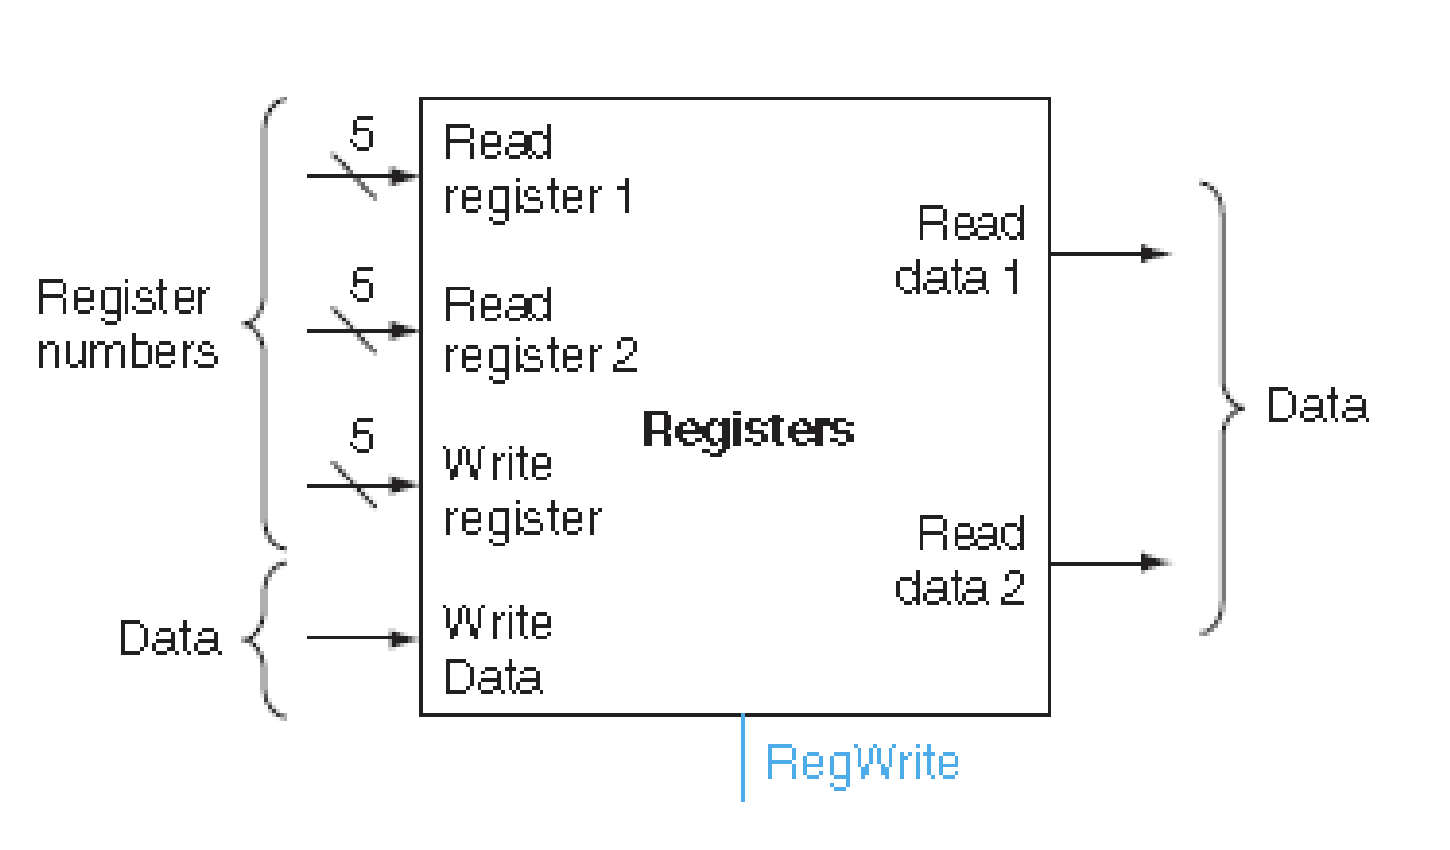
\includegraphics[width=0.8\textwidth]{./register.png}
    \caption{寄存器模块的输入输出端口示意图}
    \label{register}
\end{figure}

对于读取操作,寄存器会立刻响应,根据Read register1和Read register2中的值以及寄存器中的数据输出相应的结果。对于写入操作,由于不确定Write register、Write Data、RegWrite信号的先后顺序,为了避免发生写入错误,所以将时钟的下降沿设置为写入操作的同步信号。即只有在时钟的下降沿且regWrite信号为高电平的时候才讲Write Data的值写入Write register所对应的寄存器。
\textbf{除此以外,}还需要添加一个Reset信号输入,当其取值为1的时候要清空寄存器,为了保持同步,将清零的过程也放在时钟的下降沿和写操作合并在一起。

寄存器模块的输入输出端口示意图如图\ref{register}所示。本图来自于Lab04的实验指导书。此模块和Lab05基本一致。

\subsection{数据存储器(Data Memory)的原理}
数据存储器的功能是存储海量数据,同时支持数据的读取与写入,其输入输出端口如图\ref{datamemory}所示。本图来自于Lab04的实验指导书。

值得注意的是Address输入端口为32位,可以表示$2^{32}$个存储单元。但结合操作系统的内存相关的知识,内存的容量是有限的,32位的长度有一部分是表示页表的编号,同时由于虚拟内存的存在,导致了实际的物理内存其实远小于这个数字。在这里我仅考虑了64个存储单元,只有存储单元编号满足设定要求,即0~63才能正确访问。超出该范围的编号将不执行写操作,同时读操作也会返回0。

在该模块中,当MemWrite信号为高电平时,将WriteData的值写入Address所对应的存储单元。当MemRead信号为高电平时,将Address所对应的存储单元的值输出至ReadData。当MemWrite和MemRead信号均为低电平时,不执行任何操作。
\begin{figure}[!h]
    \centering
    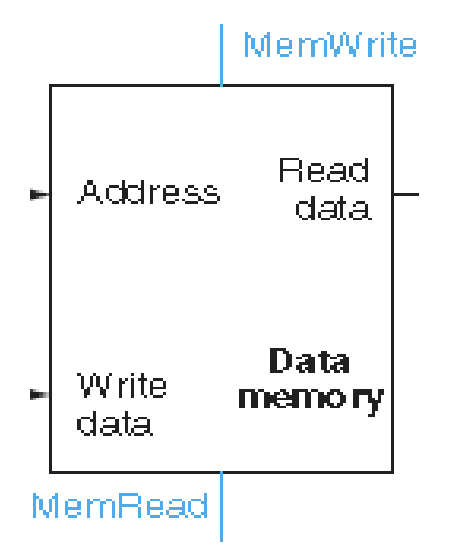
\includegraphics[width=0.5\textwidth]{./datamemory.png}
    \caption{数据存储器模块的输入输出端口示意图}
    \label{datamemory}
\end{figure}


\subsection{有符号扩展单元(Sign Extension)的原理}

有符号扩展单元的主要功能是将16位立即数扩展为32位立即数,并且根据extSign是否为1来进行有符号扩展/无符号扩展。若extSign为1,那么进行有符号扩展。在输出的32位中,高16位全部都是输入的16位有符号数的符号位,而低16位就是输入的16位符号数本身。若extSign为0,那么进行无符号扩展,输出的32位立即数的高16位全部为0,低16位为原本输入的16位立即数。其输入输出端口如图\ref{signextention}所示。本图来自于Lab04的实验指导书。
此模块和Lab05基本一致。
\begin{figure}[!h]
    \centering
    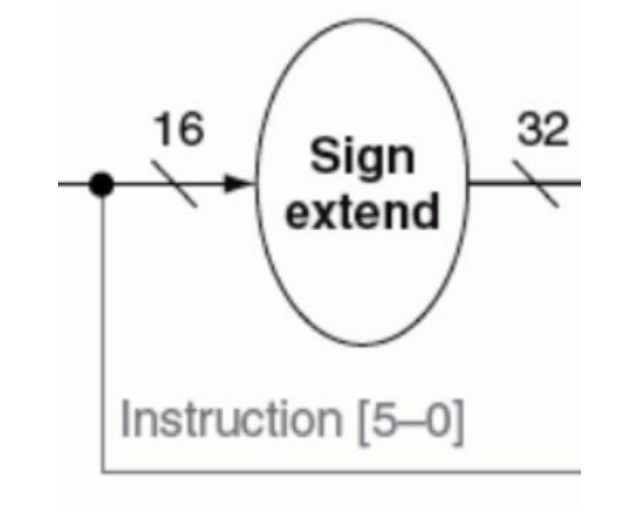
\includegraphics[width=0.6\textwidth]{./signext.png}
    \caption{有符号扩展单元模块的输入输出端口示意图}
    \label{signextention}
\end{figure}

\subsection{指令存储器(Instruction Memory)的原理}
指令存储器的输入Read address是32位的地址,输出的是其所指向的一条32位的指令Instruction[31 : 0]。其输入输出端口如图\ref{instructionmemory}所示,本图来自于Lab05的实验指导书。此模块和Lab05基本一致。
\begin{figure}[!h]
    \centering
    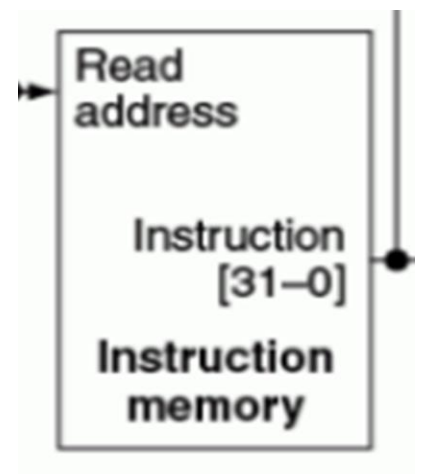
\includegraphics[width=0.5\textwidth]{./instmem.png}
    \caption{指令存储器模块的输入输出端口示意图}
    \label{instructionmemory}
\end{figure}

\subsection{多路选择器(Mux)的原理}
多路选择器的主要功能是从输入中选择其中之一输出。如图\ref{mux}所示,多路选择器有两个输入INPUT1和INPUT2。如果另外一个输入SEL的取值为1,那么输出信号OUT的取值为INPUT1,反之如果SEL的取值为0,那么输出信号OUT的取值为INPUT0。
本图来自于Lab05的实验指导书。此模块和Lab05基本一致。
\begin{figure}[!h]
    \centering
    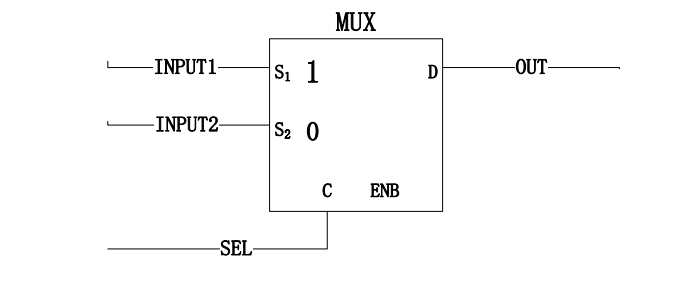
\includegraphics[width=0.6\textwidth]{./mux.png}
    \caption{多路选择器的输入输出端口示意图}
    \label{mux}
\end{figure}

在本实验中设计了两种不同的多路选择器,一种的输入输出均为32位,另外一种的输入输出均为5位。后者的使用对象是寄存器,因为一共有32个寄存器可以用5个二进制位来表示。

\subsection{程序计数寄存器(PC)的原理}
程序计数寄存器是用来管理程序地址,即PC(program counter)的模块。它在时钟的上升沿将输入pcIn写入程序计数寄存器。输出的pcOut是当前PC所在的位置,需要与程序计数寄存器的值时刻保持一致。除此以外,当Reset取值为1的时候,需要将寄存器清零。
此模块和Lab05基本一致。

\subsection{顶层模块(Top)的原理}
\subsubsection{基本通路}
顶层模块,顾名思义就是作为统领将之前设计的所有零散的子模块串联在一起,以实现单周期处理器的功能。在顶层模块的连线中包含了数据通路和控制通路,前者用于在模块之间传输数据,后者用于在模块之间传输控制信号。两者缺一不可。如图\ref{datapath}所示为单周期处理器的数据通路和控制通路。\footnote{图片来自邓倩妮老师课件,https://oc.sjtu.edu.cn/courses/52843/files/6621677?module_item_id=947833}
实现过程中的连线将按照图中示意进行。

在本实验中,还需要在此图的基础上添加段寄存器,用于判断特定指令如beq、bne、jr等的多路选择器,以及为了解决数据冒险且提高流水线效率引入的前向传递机制,暂停机制以及预测不转移机制。
\begin{figure}[!h]
    \centering
    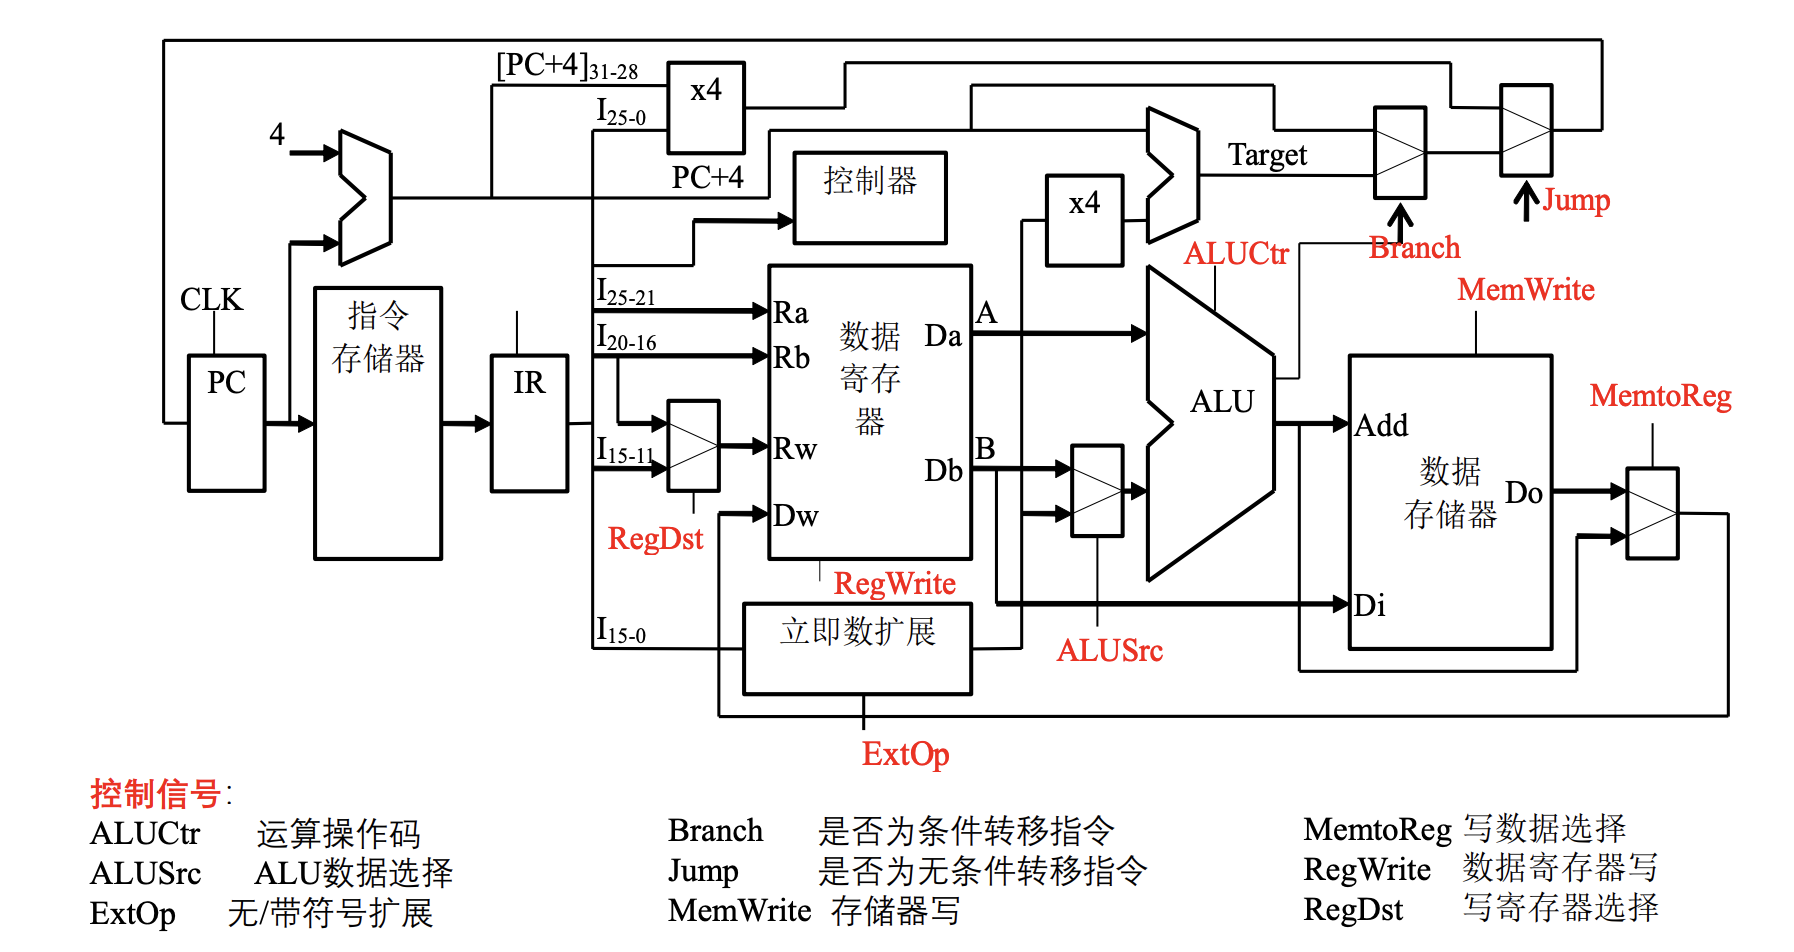
\includegraphics[width=0.8\textwidth]{./datapath.png}
    \caption{数据通路和控制通路示意图}
    \label{datapath}
\end{figure}

\subsubsection{段寄存器}
在CPU流水线的相邻两个阶段之间,需要用一个段寄存器来保存上一阶段的输出结果以及控制信号。主要有以下四个段寄存器,其功能分别与2.1节中每个阶段主要执行的任务相对应:
\begin{itemize}
    \item IF/ID段寄存器:保存IF阶段的输出结果以及控制信号,主要包含指令内容和PC的值。
    \item ID/EX段寄存器:保存ID阶段的输出结果以及控制信号,主要包含主控制器(Ctr)产生的控制信号,符号扩展模块(Sign Extension)的32位立即数输出,rs、rt寄存器的编号,写入寄存器的编号,当前PC的值等。
    \item EX/MA段寄存器:保存EX阶段的输出结果以及控制信号,主要包含算术逻辑运算单元(ALU)的运算结果,写入寄存器的编号,rt寄存器的编号等。
    \item MA/WB段寄存器:保存MA阶段的输出结果以及控制信号,主要包含写回寄存器的数据,写入寄存器的编号,以及控制是否写入的regWrite信号。
\end{itemize}

段寄存器的数据通路如图\ref{piperegister}所示,本图来自Lab06实验指导书。
\begin{figure}[!h]
    \centering
    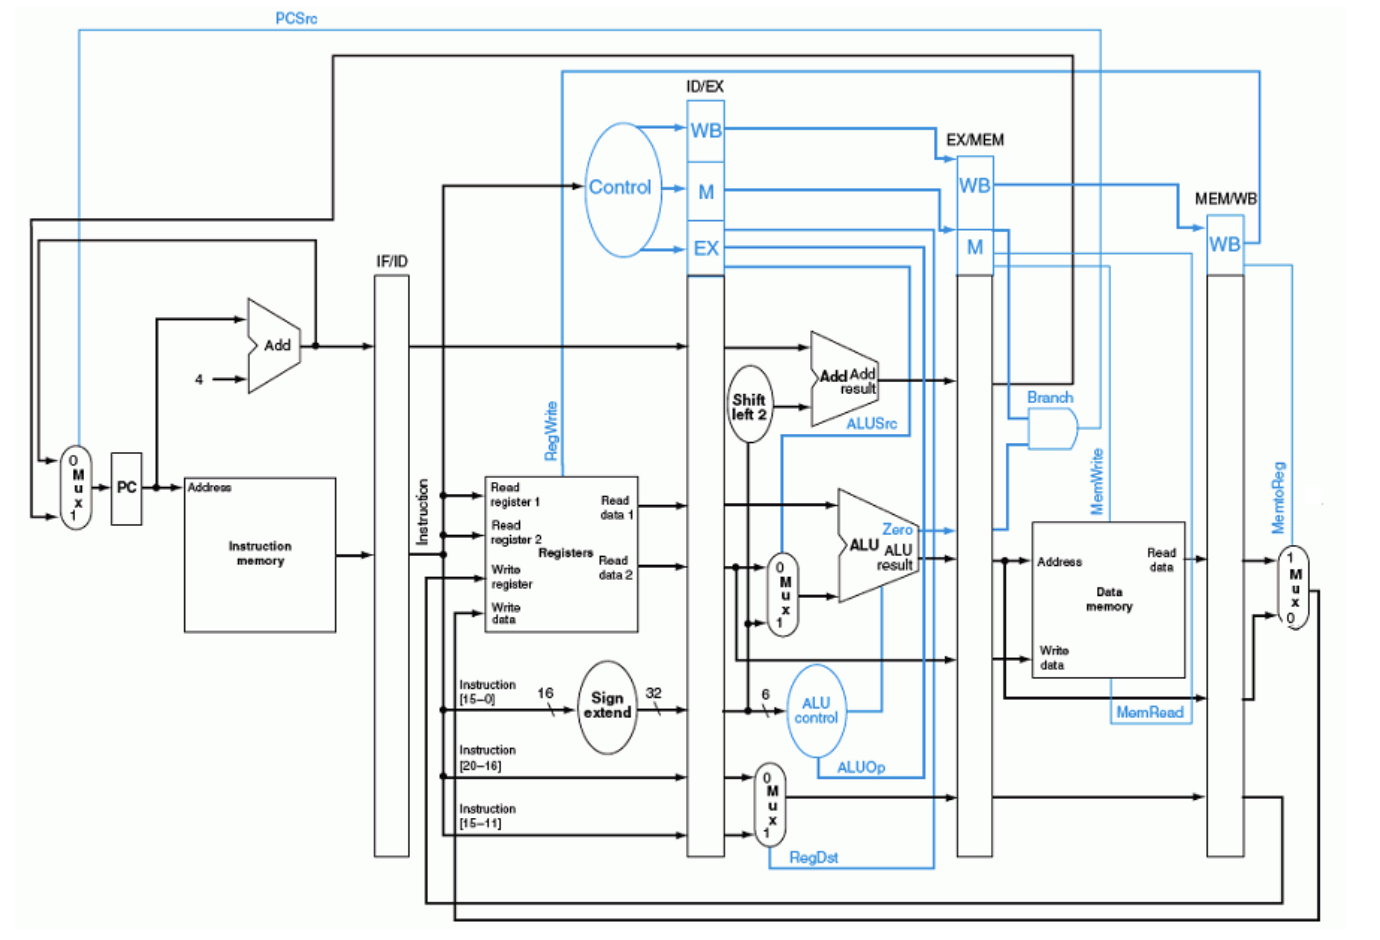
\includegraphics[width=0.8\textwidth]{./piperegister.png}
    \caption{段寄存器的数据通路}
    \label{piperegister}
\end{figure}

\subsubsection{前向传递(Forwarding)的原理}
在流水线中,当前指令在执行阶段(EX)所需要的数据可能来自先前指令的写回结果,即可能需要等到某条相关指令执行完写回操作(WB)才能继续进行。但那条指令可
能才刚开始访存阶段(MA)或写回阶段(WB)。等待该指令执行完再继续执行当前指令会导致大量流水线停滞,大大降低处理器效率。通过添加前向数据通路,从 EX/MA
段寄存器、MA/WB 段寄存器就可以获得需要的数据,避免了耗时的等待,由此提高流水线效率。


\subsubsection{停顿(Stall)的原理}
对于“load and use”型数据冒险,即lw指令,前向传递无法避免停顿,这是由于lw指令需要在访存阶段(MA)\textbf{完成
后}才能得到需要的数据,而下一条指令必须在执行阶段(EX)\textbf{开始前}获得需要的数据。因此,后一条指令必须
在执行阶段(EX)开始前暂停一个周期,等待lw指令完成访存阶段(MA)后,使用EX/MA前向数据通路使得在执行阶段(EX)能够访问到所需的数据。
在每条指令的译码阶段(ID),程序均会检测该指令是否和前一条指令形成“load and use”型数据冒险,如果存在冒险,则发出 STALL 信号暂停一个周期。

\subsubsection{转移预测(predict-not-taken)的原理}
对于跳转指令,我们通过预测不转移 (predict-not-taken) 来解决条件转移带来的控制竞争,当预测错误时,则清楚转移指令后的指令以及相关寄存器并且转移至正确的地址执行。接下来分无条件跳转指令和条件跳转指令两种情况讨论其合理性。这种策略的正确
性需要分情况说明。首先是\textbf{无条件跳转指令},在2.1.2节中提到诸如j、jal、jr这类无条件跳转指令将在译码阶段(ID)完成所有操作,包括跳转。假设发生预测错误,那么会清除ID/EX寄存器。但是此时整个跳转指令已经完成,即使清除也不会造成跳转错误。其次是\textbf{条件跳转指令}。这类指令会在执行阶段(EX)完成跳转,所以当发生预测错误的时候,此时在执行阶段(EX)之后,清除取指令阶段(IF)和译码阶段(ID)的指令是合理的,会影响至多之后的两条指令。

\section{功能实现}

\subsection{主控制器(Ctr)的功能实现}
在2.2节中已经详细介绍了主控制器实现背后的原理。与Lab05中实现主控制器模块的想法相似,在这里仍然是对输入的opCode进行判断,然后根据不同的opCode输出不同的控制信号。不同之处在于这里的模块中多了BeqSign、BneSign、LuiSign、JrSign,少了Branch。具体代码如下,仍然使用case语句进行判断。
因为代码十分长,所以只选择了一部分具有典型输出信号值的情况进行展示。
\begin{lstlisting}[language=Verilog]
    always @(opCode or funct)
    begin
        case(opCode)
        6'b000000:                  // R type instructions
        begin
            RegDst = 1;
            ALUSrc = 0;
            MemToReg = 0;
            MemRead = 0;
            MemWrite = 0;
            BeqSign = 0;
            BneSign = 0;
            ExtSign = 0;
            LuiSign = 0;
            JalSign = 0;
            ALUOp = 3'b101;
            JumpSign = 0;
            if (funct == 6'b001000) begin   
                RegWrite = 0;
                JrSign = 1;         // jr
            end else begin
                RegWrite = 1;
                JrSign = 0;
            end
        end
        6'b100011:                  // lw
        begin
            RegDst = 0;
            ALUSrc = 1;
            MemToReg = 1;
            RegWrite = 1;
            MemRead = 1;
            MemWrite = 0;
            BeqSign = 0;
            BneSign = 0;
            ExtSign = 1;
            LuiSign = 0;
            JalSign = 0;
            ALUOp = 3'b000;
            JumpSign = 0;
            JrSign = 0;
        end
        6'b101011:                  //sw
        begin
            RegDst = 0; 
            ALUSrc = 1;
            MemToReg = 0;  
            RegWrite = 0;
            MemRead = 0;
            MemWrite = 1;
            BeqSign = 0;
            BneSign = 0;
            ExtSign = 1;
            LuiSign = 0;
            JalSign = 0;
            ALUOp = 3'b000;
            JumpSign = 0;
            JrSign = 0;
        end
        6'b000100:                  // beq
        begin
            RegDst = 0; 
            ALUSrc = 0;
            MemToReg = 0;  
            RegWrite = 0;
            MemRead = 0;
            MemWrite = 0;
            BeqSign = 1;            // BeqSign is 1
            BneSign = 0;
            ExtSign = 1;
            LuiSign = 0;
            JalSign = 0;
            ALUOp = 3'b001;
            JumpSign = 0;
            JrSign = 0;
        end
        6'b000101:                  // bne
        begin
            RegDst = 0; //x
            ALUSrc = 0;
            MemToReg = 0;   //x
            RegWrite = 0;
            MemRead = 0;
            MemWrite = 0;
            BeqSign = 0;
            BneSign = 1;            // BneSign is 1
            ExtSign = 1;
            LuiSign = 0;
            JalSign = 0;
            ALUOp = 3'b001;
            JumpSign = 0;
            JrSign = 0;
        end
        6'b000010:                  // jump
        begin
            RegDst = 0;
            ALUSrc = 0;
            MemToReg = 0;
            RegWrite = 0;
            MemRead = 0;
            MemWrite = 0;
            BeqSign = 0;
            BneSign = 0;
            ExtSign = 0;
            LuiSign = 0;
            JalSign = 0;
            ALUOp = 3'b000;
            JumpSign = 1;           // JumpSign is 1
            JrSign = 0;
        end
        6'b001000:                  // addi
        begin
            RegDst = 0;
            ALUSrc = 1;
            MemToReg = 0;
            RegWrite = 1;
            MemRead = 0;
            MemWrite = 0;
            BeqSign = 0;
            BneSign = 0;
            ExtSign = 1;
            LuiSign = 0;
            JalSign = 0;
            ALUOp = 3'b000; //add
            JumpSign = 0;
            JrSign = 0;
        end
        6'b001110:                  // xori
        begin
            RegDst = 0;
            ALUSrc = 1;
            MemToReg = 0;
            RegWrite = 1;
            MemRead = 0;
            MemWrite = 0;
            BeqSign = 0;
            BneSign = 0;
            ExtSign = 0;
            LuiSign = 0;
            JalSign = 0;
            ALUOp = 3'b111;
            JumpSign = 0;
            JrSign = 0;
        end
        6'b001111:                  // lui
        begin
            RegDst = 0;
            ALUSrc = 0;
            MemToReg = 0;
            RegWrite = 1;
            MemRead = 0;
            MemWrite = 0;
            BeqSign = 0;
            BneSign = 0;
            ExtSign = 0;
            LuiSign = 1;            // LuiSign is 1
            JalSign = 0;
            ALUOp = 3'b000;
            JumpSign = 0;
            JrSign = 0;
        end
        6'b001010:                  // slti
        begin
            RegDst = 0;
            ALUSrc = 1;
            MemToReg = 0;
            RegWrite = 1;
            MemRead = 0;
            MemWrite = 0;
            BeqSign = 0;
            BneSign = 0;
            ExtSign = 1;
            LuiSign = 0;
            JalSign = 0;
            ALUOp = 3'b010;
            JumpSign = 0;
            JrSign = 0;
        end
        default:
        begin
            RegDst = 0;
            ALUSrc = 0;
            MemToReg = 0;
            RegWrite = 0;
            MemRead = 0;
            MemWrite = 0;
            ALUOp = 2'b00;
            JumpSign = 0;
            JrSign = 0;
        end
        endcase
    end

\end{lstlisting}

\subsection{运算单元控制器(ALUCtr)的功能实现}
在2.3节中已经详细介绍了运算单元控制器实现背后的原理。与Lab05中实现主控制器模块的想法相似,在这里仍然是对输入的aluOp和Funct先位拼接然后再进行判断,根据不同的组合输出不同的AluCtrOut。
不同之处在于因为JrSign在主控制器模块产生,所以此处不再需要了。同时因为本处理器将支持的16条指令扩展为31条,所以需要增加扩展出来的指令的判断。具体代码如下。因为拼接后存在通配符X,所以仍然使用casex语句进行判断。

\begin{lstlisting}[language=Verilog]
    always @ (aluOp or funct)
    begin
    // Initialization of "Sign of shift amount"
        ShamtSign = 0;
    // switch case 
        casex({aluOp,funct})
            9'b000xxxxxx:                   // lw, sw, add, addiu
                ALUCtrOut = 4'b0010;    
            9'b001xxxxxx:                   // beq, bne
                ALUCtrOut = 4'b0110;    
            9'b010xxxxxx:                   // slti
                ALUCtrOut = 4'b0111;
            9'b110xxxxxx:                   // sltiu
                ALUCtrOut = 4'b1000;
            9'b011xxxxxx:                   // andi
                ALUCtrOut = 4'b0000;
            9'b100xxxxxx:                   // ori
                ALUCtrOut = 4'b0001;
            9'b111xxxxxx:                   // xori
                ALUCtrOut = 4'b1011;
            9'b101001000:                   // jr
                ALUCtrOut = 4'b0101;

            // Shift amount related are as below
            9'b101000000:                   // sll
            begin
                ALUCtrOut = 4'b0011;
                ShamtSign = 1;
            end
            9'b101000010:                   // srl
            begin
                ALUCtrOut = 4'b0100;
                ShamtSign = 1;
            end
            9'b101000011:                   // sra
            begin
                ALUCtrOut = 4'b1110;
                ShamtSign = 1;
            end
            9'b101100000:                   // add
                ALUCtrOut = 4'b0010;
            9'b101100011:                   // subu
                ALUCtrOut = 4'b0110;
            9'b101100100:                   // and
                ALUCtrOut = 4'b0000;
            9'b101100101:                   // or
                ALUCtrOut = 4'b0001;
            9'b101100110:                   // xor
                ALUCtrOut = 4'b1011;
            9'b101100001:                   // addu
                ALUCtrOut = 4'b0010;
            9'b101100010:                   // sub
                ALUCtrOut = 4'b0110;
            9'b101100111:                   // nor
                ALUCtrOut = 4'b1100;
            9'b101101010:                   // slt
                ALUCtrOut = 4'b0111;
            9'b101101011:                   // sltu
                ALUCtrOut = 4'b1000;
            9'b101000100:                   // sllv
                ALUCtrOut = 4'b0011;
            9'b101000110:                   // srlv
                ALUCtrOut = 4'b0100;
            9'b101000111:                   // srav
                ALUCtrOut = 4'b1110;
        endcase
    end
    
   
\end{lstlisting}

\subsection{算术逻辑运算单元(ALU)的功能实现}
在2.3节中已经详细介绍了算数逻辑运算单元实现背后的原理。与Lab05中实现主控制器模块的想法相似,在这里仍然是对输入的aluCtrOut进行判断,从而对两个输入input1和input2进行相应的算数操作。最后根据结果ALURes是否为0来判断是否需要将Zero置1。具体代码如下。

值得注意的是Verilog会自动把wire类型解释为无符号数,因此想进行有符号的运算时,必须进行强制类型转换,即在需要转换的变量外面套上\texttt{\$signed()}。
\begin{lstlisting}[language=Verilog]
    always @ (input1 or input2 or aluCtrOut)
    begin
        case(aluCtrOut)
        4'b0000:                        // and
            ALURes = input1 & input2;
        4'b0001:                        // or
            ALURes = input1 | input2;
        4'b0010:                        // add
            ALURes = input1 + input2;
        4'b0011:                        // left shift
            ALURes = input2 << input1;
        4'b0100:                        // right shift
            ALURes = input2 >> input1;
        4'b0110:                        // sub
            ALURes = input1 - input2;
        4'b0111:                        // slt signed
            ALURes = (input1 < input2);
        4'b1000:                        // slt unsigned
            ALURes = ($signed(input1) < $signed(input2));
        4'b1011:                        // xor
            ALURes = input1 ^ input2;
        4'b1100:                        // nor
            ALURes = ~(input1 | input2);
        4'b1110:                        // shift right arithmetic
            ALURes = ($signed(input2) >> input1);
        endcase
        if(ALURes==0)
            Zero = 1;
        else
            Zero = 0;
    end

\end{lstlisting}

\subsection{寄存器(Register)的功能实现}
在2.4节中已经详细介绍了寄存器实现背后的原理。寄存器的实现与Lab04基本一致,唯一的区别在于在这里需要添加Reset信号,当其值为1的时候,要清空寄存器。具体代码如下。

\begin{lstlisting}[language=Verilog]
module Registers(
    input [25 : 21] readReg1,
    input [20 : 16] readReg2,
    input [4 : 0] writeReg,
    input [31 : 0] writeData,
    input regWrite,
    input reset,
    input clk,
    output reg [31 : 0] readData1,
    output reg [31 : 0] readData2
    );
    
    reg [31:0] RegFile[31:0];
    // Initialization of RegFile 
    integer i;
    initial begin
        RegFile[0] = 0;
    end

    always @ (readReg1 or readReg2) begin
        begin
        readData1 = RegFile[readReg1];
        readData2 = RegFile[readReg2];
        end
    end

    always @ (negedge clk or reset)
    begin
        if(reset)                               // reset the register
        begin
            for(i = 0; i < 32; i = i + 1)
                RegFile[i] = 0;
        end
        else begin
            if(regWrite)
                RegFile[writeReg] = writeData; 
        end
    end

endmodule
\end{lstlisting}

\subsection{数据存储器(Data Memory)的功能实现}
在2.5节已经详细介绍了数据存储器的原理。对于写入操作将由时钟的下降沿进行同步,将WriteData的值写入Address所对应的存储单元。对于读操作,每当memRead这个读操作的标志以及address发生改变的时候,就需要重新读取address所指向的内存空间的数据,并将其输出。具体代码如下。
\begin{lstlisting}[language=Verilog]
module dataMemory (
    input clock,
    input [31 : 0] address,
    input [31 : 0] writeData,
    input memWrite,
    input memRead,
    output [31 : 0] readData
);    
    reg [31 : 0] memFile [0 : 63];
    reg [31 : 0] ReadData;
    integer i;
    
    // initialization
    initial begin
    ReadData = 0;
    for (i = 0; i < 64; i=i+1)
        memFile[i]=0;
    end
    
    // Read operation is performed when memRead is high
    always @ (address or memRead) 
        begin
            if (memRead == 1)
                if (address <= 63)               // address less than 64 is valid
                    ReadData = memFile[address];
                 else                            // invalid address
                    ReadData = 0;
          
        end
    
    // Write operation is performed when memWrite is high
    always @ (negedge clock) 
        begin
            if (memWrite == 1 && address <= 63) 
                memFile[address] = writeData;
        end
        
    assign readData = ReadData
    endmodule    
\end{lstlisting}

\subsection{有符号扩展单元(Sign Extension)的功能实现}
在2.6节已经详细介绍了有符号扩展单元的原理。与Lab04中的实现类似,仍然采用三目运算符\texttt{?:}来简化代码。不同之处在于需要额外加入extSign信号用于判断是否需要有符号扩展即可。具体代码如下。

\begin{lstlisting}[language=Verilog]
    module signext(
    input [15 : 0] inst,
    input signExt,
    output [31 : 0] data
    );
    assign data = (signExt) ? {{16{inst[15]}},inst[15:0]} : {{16{0}},inst[15:0]};
\end{lstlisting}

\subsection{指令存储器(Instruction Memory)的功能实现}
在2.7节已经详细介绍了指令存储器的原理。它仅仅只需要根据输入的地址去输出所对应的指令即可。为了整体的鲁棒性,还需判断地址是否有效,若不在有效范围之内,那么就将结果置0。具体代码如下。
\begin{lstlisting}[language=Verilog]
module InstMemory(
        input[31 : 0] address,
        output[31 : 0] instructiion
    );

    reg [31 : 0] instFile[0 : 63];
    // check for validity of address
    assign instructiion = ((address / 4) <= 63) ? instFile[address / 4] : 0;
endmodule
\end{lstlisting}

\subsection{多路选择器(Mux)的功能实现}
在2.8节已经详细介绍了多路选择器的原理。使用三目运算符就可以轻松的实现从两个输入中选择一个输出的功能。同时支持32位二进制数的多路选择器和支持5位二进制数的多路选择器的唯一区别就在于输入的位数不同,在实现逻辑上无任何差异。具体代码如下。
\begin{lstlisting}[language=Verilog]
module Mux(
    input [31:0] input0,
    input [31:0] input1,
    input select,
    output [31:0] out
    );
    assign out = select ? input1 : input0;
endmodule
\end{lstlisting}

\subsection{程序计数模块(PC)的功能实现}
在2.9节已经详细介绍了程序计数模块的原理。在实现的过程中,在时钟的上边缘将输入pcIn写进寄存器。除此以外,如果reset的值为1,那么PC的值将置0。除此以外,输出pcOut的值始终得和寄存器中的值保持一致,那么就需要用到assign语句。具体代码如下。
\begin{lstlisting}[language=Verilog]
module PC(
    input [31:0] pcIn,
    input clk,
    input reset,
    output [31:0] pcOut
);
    
initial begin
    PC = 0;
end

always @ (posedge clk or reset)
    begin
        if(reset == 1)
            PC = 0;                 // PC needs to be reset
        else
            PC = pcIn;
    end
assign pcOut = PC;                  // pcOut keeps synchronized with PC
endmodule
\end{lstlisting}

\subsection{顶层模块(Top)的功能实现}
由于顶层模块的组成很复杂,我将分为段寄存器、模块实例化、前向传递的实现、流水线的实现来展开。
\subsubsection{段寄存器}
值得一提的是在编写代码的时候并不需要将所有的段寄存器全部定义在一起,最好是在每个阶段前定义该阶段对应的段寄存器,方便使用。
\begin{lstlisting}[language=Verilog]
    // IF/ID Registers
    reg [31 : 0] IF_TO_ID_INST;
    reg [31 : 0] IF_TO_ID_PC;

    // ID/EX Registers
    reg [2 : 0] ID_TO_EX_ALUOP;
    reg [7 : 0] ID_TO_EX_CTR_SIGNALS;
    reg [31 : 0] ID_TO_EX_EXT_RES;
    reg [4 : 0] ID_TO_EX_INST_RS;        
    reg [4 : 0] ID_TO_EX_INST_RT;        
    reg [31 : 0] ID_TO_EX_REG_READ_DATA1;
    reg [31 : 0] ID_TO_EX_REG_READ_DATA2;
    reg [5 : 0] ID_TO_EX_INST_FUNCT;
    reg [4 : 0] ID_TO_EX_INST_SHAMT;
    reg [4 : 0] ID_TO_EX_REG_DEST;
    reg [31 : 0] ID_TO_EX_PC;

    // EX/MA Registers
    reg [3 : 0] EX_TO_MA_CTR_SIGNALS;
    reg [31 : 0] EX_TO_MA_ALU_RES;
    reg [31 : 0] EX_TO_MA_REG_READ_DATA_2;
    reg [4 : 0] EX_TO_MA_REG_DEST;

    // MA/WB Registers
    reg MA_TO_WB_CTR_SIGNALS;
    reg [31 : 0] MA_TO_WB_FINAL_DATA;
    reg [4 : 0] MA_TO_WB_REG_DEST;
\end{lstlisting}

\subsubsection{子模块初始化}
此部分与Lab05类似,模块的实例化方法仍然是用类似于\texttt{.opCode(OPCODE)}的方式,这样可以避免模块内的变量顺序和实例化时的数据顺序不一致导致的问题。具体代码如下。
值得注意的是跳转指令所对应的多路选择器的初始化,在2.1节中已经说明对于无条件跳转指令如j、jr,跳转将在ID阶段完成,而对于条件跳转指令是在EX阶段后才执行完。因此在实例化模块时可以放在每个阶段所对应的代码段中。
\begin{lstlisting}[language=Verilog]

    wire [12 : 0] ID_CTR_SIGNALS;
    wire [2 : 0] ID_CTR_SIGNAL_ALUOP;
    wire ID_JUMP_SIGN;
    wire ID_JR_SIGN;
    wire ID_EXT_SIGN;
    wire ID_REG_DST_SIGN;
    wire ID_JAL_SIGN;
    wire ID_ALU_SRC_SIGN;
    wire ID_LUI_SIGN;
    wire ID_BEQ_SIGN;
    wire ID_BNE_SIGN;
    wire ID_MEM_WRITE_SIGN;
    wire ID_MEM_READ_SIGN;
    wire ID_MEM_TO_REG_SIGN;
    wire ID_REG_WRITE_SIGN;
    wire ID_ALU_OP;
    // In ID stage, initialize Ctr module
    Ctr ctr(
        .opCode(IF_TO_ID_INST[31:26]),
        .funct(IF_TO_ID_INST[5:0]),
        .jumpSign(ID_JUMP_SIGN),
        .jrSign(ID_JR_SIGN),
        .extSign(ID_EXT_SIGN),
        .regDst(ID_REG_DST_SIGN),
        .jalSign(ID_JAL_SIGN),
        .aluSrc(ID_ALU_SRC_SIGN),
        .luiSign(ID_LUI_SIGN),
        .beqSign(ID_BEQ_SIGN),
        .bneSign(ID_BNE_SIGN),
        .memWrite(ID_MEM_WRITE_SIGN),
        .memRead(ID_MEM_READ_SIGN),
        .memToReg(ID_MEM_TO_REG_SIGN),
        .regWrite(ID_REG_WRITE_SIGN),
        .aluOp(ID_CTR_SIGNAL_ALUOP)
    );

    wire[31 : 0] ID_REG_READ_DATA1;                     
    wire[31 : 0] ID_REG_READ_DATA2;                 
    wire[4 : 0] WB_WRITE_REG_ID;         
    wire[4 : 0] WB_WRITE_ID;              // Register ID used to write back after jal mux
    wire[31 : 0] WB_REG_WRITE_DATA;       
    wire[31 : 0] WB_REG_DATA;             // Data written back after jal mux
    wire WB_REG_WRITE;          
    wire [4 : 0] ID_REG_DEST;
    wire [4 : 0] ID_REG_RS = IF_TO_ID_INST[25 : 21];
    wire [4 : 0] ID_REG_RT = IF_TO_ID_INST[20 : 16];
    wire [4 : 0] ID_REG_RD = IF_TO_ID_INST[15 : 11];

    Mux jal_data_mux(
        .select(ID_JAL_SIGN),
        .input0(WB_REG_WRITE_DATA),
        .input1(IF_TO_ID_PC + 4),
        .out(WB_REG_DATA)
    );

    Mux jal_reg_id_mux(
        .select(ID_JAL_SIGN),
        .input0(WB_WRITE_REG_ID),
        .input1(5'b11111),
        .out(WB_WRITE_ID)
    );
    
    // As illustrated in 2.1.2, we need to determine the write back register in ID stage
    // Register takes only 5 bits to denote, so we use 5-bit mux
    Mux_5bits reg_dst_mux(
        .select(ID_CTR_SIGNALS[9]),
        .input0(ID_REG_RT),
        .input1(ID_REG_RD),
        .out(ID_REG_DEST)
    );

    Registers reg_file(
        .readReg1(ID_REG_RS),
        .readReg2(IF_TO_ID_INST[20:16]),
        .writeReg(WB_WRITE_ID),
        .writeData(WB_REG_DATA),
        .regWrite(WB_REG_WRITE),
        .clk(clk),
        .reset(reset),
        .readData1(ID_REG_READ_DATA1),
        .readData2(ID_REG_READ_DATA2)
    );
    
    wire [31:0] ID_EXT_RES;
    // Sign extension operation also happens in ID stage
    signext sign_ext(
        .inst(IF_TO_ID_INST[15:0]),
        .signExt(ID_EXT_SIG),
        .data(ID_EXT_RES)
    );

    wire EX_ALU_SRC_SIG = ID_TO_EX_CTR_SIGNALS[7];
    wire EX_LUI_SIG = ID_TO_EX_CTR_SIGNALS[6];
    wire EX_BEQ_SIG = ID_TO_EX_CTR_SIGNALS[5];
    wire EX_BNE_SIG = ID_TO_EX_CTR_SIGNALS[4];

    wire [3:0] EX_ALU_CTR_OUT;                  // ALUCtr's output in EX stage
    wire EX_SHAMT_SIGN;                         // shift amount sign in EX stage

    // In EX stage, modules relative to ALU will be initialized, such as ALUCtr, ALU

    ALUCtr alu_ctr(
        .aluOp(ID_TO_EX_ALUOP),
        .funct(ID_TO_EX_INST_FUNCT),
        .shamtSign(EX_SHAMT_SIGN),
        .aluCtrOut(EX_ALU_CTR_OUT)
    );

    wire EX_ALU_ZERO;                             // Zero sign in ALU module
    wire [31 : 0] EX_ALU_RES;                     // ALU's result
    wire [31 : 0] EX_LUI_DATA;                    // Special case for LUI instruction
    ALU alu(
        .input1(EX_ALU_INPUT1),
        .input2(EX_ALU_INPUT2),
        .aluCtr(EX_ALU_CTR_OUT),
        .aluRes(EX_ALU_RES),
        .zero(EX_ALU_ZERO)
    );

    // Recall in 2.1.3, we have stated that for lui, it needs to throw the output of ALU

    Mux lui_mux(
        .select(EX_LUI_SIGN),
        .input0(EX_ALU_RES),
        .input1({ID_TO_EX_EXT_RES[15 : 0], 16'b0}),
        .out(EX_LUI_DATA)
    );

    // In MA stage, modules related to Memory are initialized

    wire MA_MEM_WRITE = EX_TO_MA_CTR_SIGNALS[3];
    wire MA_MEM_READ = EX_TO_MA_CTR_SIGNALS[2];
    wire MA_MEM_TO_REG = EX_TO_MA_CTR_SIGNALS[1];
    wire MA_REG_WRITE = EX_TO_MA_CTR_SIGNALS[0];

    
    wire [31:0] MA_OUTPUT_DATA;
    // As is illustrated in 2.1.4, instruction may have access to memory in MA stage
    // Need to choose between result of ALU or data from memory to output
    Mux mem_to_reg_mux(
        .input0(EX_TO_MA_ALU_RES),
        .input1(MA_MEM_READ_DATA),
        .select(MA_MEM_TO_REG),
        .out(MA_OUTPUT_DATA)
    );

    // The following is the Initialization of SHIFT instructions, including JUMP, JR, BNE, BEQ

    // Recall thayt UNCONDITIONAL SHIFT will finish in ID stage !!! Including J and JR !
    wire[31 : 0] PC_AFTER_JUMP_MUX;
    Mux jump_mux(
        .select(ID_JUMP_SIGN), 
        .input1(((IF_TO_ID_PC + 4) & 32'hf0000000) + (IF2ID_INST [25 : 0] << 2)),
        .input0(IF_PC + 4),
        .out(PC_AFTER_JUMP_MUX)
    );
    
    wire[31:0] PC_AFTER_JR_MUX;
    Mux jr_mux(
        .select(ID_JR_SIG),   
        .input0(PC_AFTER_JUMP_MUX),
        .input1(ID_REG_READ_DATA1),
        .out(PC_AFTER_JR_MUX)
    );
    
    // For CONDITIONAL SHIFT, things will happen in EX stage, including BEQ and BNE 
    wire EX_BEQ_BRANCH = EX_BEQ_SIG & EX_ALU_ZERO;
    wire[31 : 0] PC_AFTER_BEQ_MUX;
    Mux beq_mux(
        .select(EX_BEQ_BRANCH),
        .input1(BRANCH_DEST),
        .input0(PC_AFTER_JR_MUX),
        .out(PC_AFTER_BEQ_MUX)
    );
    
    wire EX_BNE_BRANCH = EX_BNE_SIG & (~ EX_ALU_ZERO);
    wire[31 : 0] PC_AFTER_BNE_MUX;
    Mux bne_mux(
        .select(EX_BNE_BRANCH),
        .input1(BRANCH_DEST),
        .input0(PC_AFTER_BEQ_MUX),
        .out(PC_AFTER_BNE_MUX)
    );
\end{lstlisting}

\subsubsection{前向传递的实现}
在2.11.3节中已经详细说明了前向传递的原理,在实现的过程中考虑到EX阶段主要处理与ALU相关的任务,而且ALU有两个输入口都可能需要前向传递的数据。所以设置了两组前项通路,其中每一组中又包含两个多路选择器,分别从EX/MA和MA/WB段寄存器中读取所需数据。同时前向传递还得满足当前的读取寄存器和先前的写入寄存器是一样的前提。具体代码如下。
\begin{lstlisting}[language=Verilog]
    wire[31:0] EX_FORWARDING_P1_TEMP;
    wire[31:0] EX_FORWARDING_P2_TEMP;
    // 1st forwarding mux pair 
    // mux1 reads from MA/WB
    Mux forward_input1_MAWB_mux1(
        .select(WB_REG_WRITE & (MA_TO_WB_REG_DEST == ID_TO_EX_INST_RS)),
        .input0(ID_TO_EX_REG_READ_DATA1),
        .input1(MA_TO_WB_FINAL_DATA),
        .out(EX_FORWARDING_P1_TEMP)
    );
    // mux2 reads from EX/MA
    Mux forward_input1_EXMA_mux2(
        .select(MA_REG_WRITE & (EX_TO_MA_REG_DEST == ID_TO_EX_INST_RS)),
        .input0(EX_FORWARDING_A_TEMP),
        .input1(EX_TO_MA_ALU_RES),
        .out(FORWARDING_RES_P1)
    );
    
    // 2nd forwarding mux pair 
    // mux1 reads from MA/WB
    Mux forward_input2_MAWB_mux1(
        .select(WB_REG_WRITE & (MA_TO_WB_REG_DEST == ID_TO_EX_INST_RT)),
        .input0(ID_TO_EX_REG_READ_DATA2),
        .input1(MA_TO_WB_FINAL_DATA),
        .out(EX_FORWARDING_P2_TEMP)
    );
    // mux2 reads from EX/MA
    Mux forward_input2_EXMA_mux2(
        .select(MA_REG_WRITE & (EX_TO_MA_REG_DEST == ID_TO_EX_INST_RT)),
        .input0(EX_FORWARDING_B_TEMP),
        .input1(EX_TO_MA_ALU_RES),
        .out(FORWARDING_RES_P2)
    );
\end{lstlisting}

\subsubsection{流水线的实现}
在这个部分,实现了转移预测、停顿、流水线等功能。在这之中段寄存器何时清空,何时产生停顿比较重要,做如下分析。
在讨论之前首先需要明确NOP信号是预测错误的标志,STALL是暂停的标志。在这里需要考虑jal这样一种特殊的指令,它的执行过程横跨所有阶段,由它引起的暂停和其他指令的暂停对寄存器是否需要清空有不同的影响。

首先是IF/ID段寄存器。当NOP信号为1时,说明转移预测有误,此时需要清空IF/ID段寄存器。

接下来是ID/EX段寄存器。当NOP信号为1时,说明转移预测有误,此时需要清空此寄存器。当STALL信号为1时,说明此时需要暂停,同样也需要清空当前的寄存器,避免暂停结束后继续执行时产生错误。若此时的指令是jal,则不需要清除ID/EX段寄存器。

最后是EX/MA段寄存器和MA/WB段寄存器。当指令是jal时,译码阶段(ID)后会暂停一个周期,此时无需清除EX/MA、MA/WB段寄存器。
\begin{lstlisting}[language=Verilog]
    always @(posedge clk) 
    begin
        // NOP stands for the circumstance where the prediction is wrong.
        // Only those Shift instructions such as j, jr, beq, bne may lead to wrong prediction.
        NOP = BRANCH | ID_JUMP_SIGN | ID_JR_SIGN;
        // STALL means that it needs to stop for a circle.
        STALL = ID_TO_EX_CTR_SIGNALS[2] & ((ID_TO_EX_INST_RT == ID_REG_RS) | (ID_TO_EX_INST_RT == ID_REG_RT)); 

        // Unless there are special cases when the registers should be emptied, registers should all be able to written into.

        // IF/ID Register 
        if(!STALL)
        begin
        // when NOP = 1, IF/ID register should be emptied.
            if(NOP)                         
            begin
                if(IF_PC == NEXT_PC)
                begin
                    IF_TO_ID_INST <= IF_INST;
                    IF_TO_ID_PC <= IF_PC;
                    IF_PC <= IF_PC + 4;
                end
                else begin
                    IF_TO_ID_INST <= 0;
                    IF_TO_ID_PC <= 0;
                    IF_PC <= NEXT_PC;
                end
            end
            else begin
                IF_TO_ID_INST <= IF_INST;
                IF_TO_ID_PC <= IF_PC;
                IF_PC <= NEXT_PC;
            end
        end
        
        // ID/EX Register
        // Recall that JAL instruction is a special case when dealing with NOP and STALL.
        // It does not need to empty any pipe registers.
        if (!ID_JAL_SIG)
        begin
        // No matter STALL or NOP, this register should be emptied.
            if (STALL | NOP)
            begin
            // For UNCONDITIONAL SHIFT like J and JR, no need to care
            // For CONDITIONAL SHIFT like BNE and BEQ, instructions should be interrupted here if something wrong happens.
                ID_TO_EX_PC <= IF2ID_PC;
                ID_TO_EX_ALUOP <= 3'b000;
                ID_TO_EX_CTR_SIGNALS <= 0;
                ID_TO_EX_EXT_RES <= 0;
                ID_TO_EX_INST_RS <= 0;
                ID_TO_EX_INST_RT <= 0;
                ID_TO_EX_REG_READ_DATA1 <= 0;
                ID_TO_EX_REG_READ_DATA2 <= 0;
                ID_TO_EX_INST_FUNCT <= 0;
                ID_TO_EX_INST_SHAMT <= 0;
                ID_TO_EX_REG_DEST <= 0;
            end else 
            begin
                ID_TO_EX_PC <= IF_TO_ID_PC;
                ID_TO_EX_ALUOP <= ID_CTR_SIGNAL_ALUOP;
                ID_TO_EX_CTR_SIGNALS <= ID_CTR_SIGNALS[7 : 0];
                ID_TO_EX_EXT_RES <= ID_EXT_RES;
                ID_TO_EX_INST_RS <= ID_REG_RS;
                ID_TO_EX_INST_RT <= ID_REG_RT;
                ID_TO_EX_REG_DEST <= ID_REG_DEST;
                ID_TO_EX_REG_READ_DATA1 <= ID_REG_READ_DATA1;
                ID_TO_EX_REG_READ_DATA2 <= ID_REG_READ_DATA2;
                ID_TO_EX_INST_FUNCT <= IF_TO_ID_INST[5 : 0];
                ID_TO_EX_INST_SHAMT <= IF_TO_ID_INST[10 : 6];
            end
        end

        // EX/MA
        // Again, special case for JAL instruction.
        if (!ID_JAL_SIG)
        begin
            EX_TO_MA_CTR_SIGNALS <= ID_TO_EX_CTR_SIGNALS[3 : 0];
            EX_TO_MA_ALU_RES <= EX_FINAL_DATA;
            EX_TO_MA_REG_READ_DATA_2 <= FORWARDING_RES_B;
            EX_TO_MA_REG_DEST <= ID_TO_EX_REG_DEST;
        end

        // MA/WB
        // Again, special case for JAL instruction.
        if (!ID_JAL_SIG)
        begin
            MA_TO_WB_CTR_SIGNALS <= EX_TO_MA_CTR_SIGNALS[0];
            MA_TO_WB_FINAL_DATA <= MA_FINAL_DATA;
            MA_TO_WB_REG_DEST <= EX_TO_MA_REG_DEST;
        end
        
    end
\end{lstlisting}

\section{结果验证}
在仿真验证时,我采用了微信群中分享的指令集和数据集,如图\ref{instruction},\ref{initialization}所示。
\begin{figure}[!h]
    \centering
    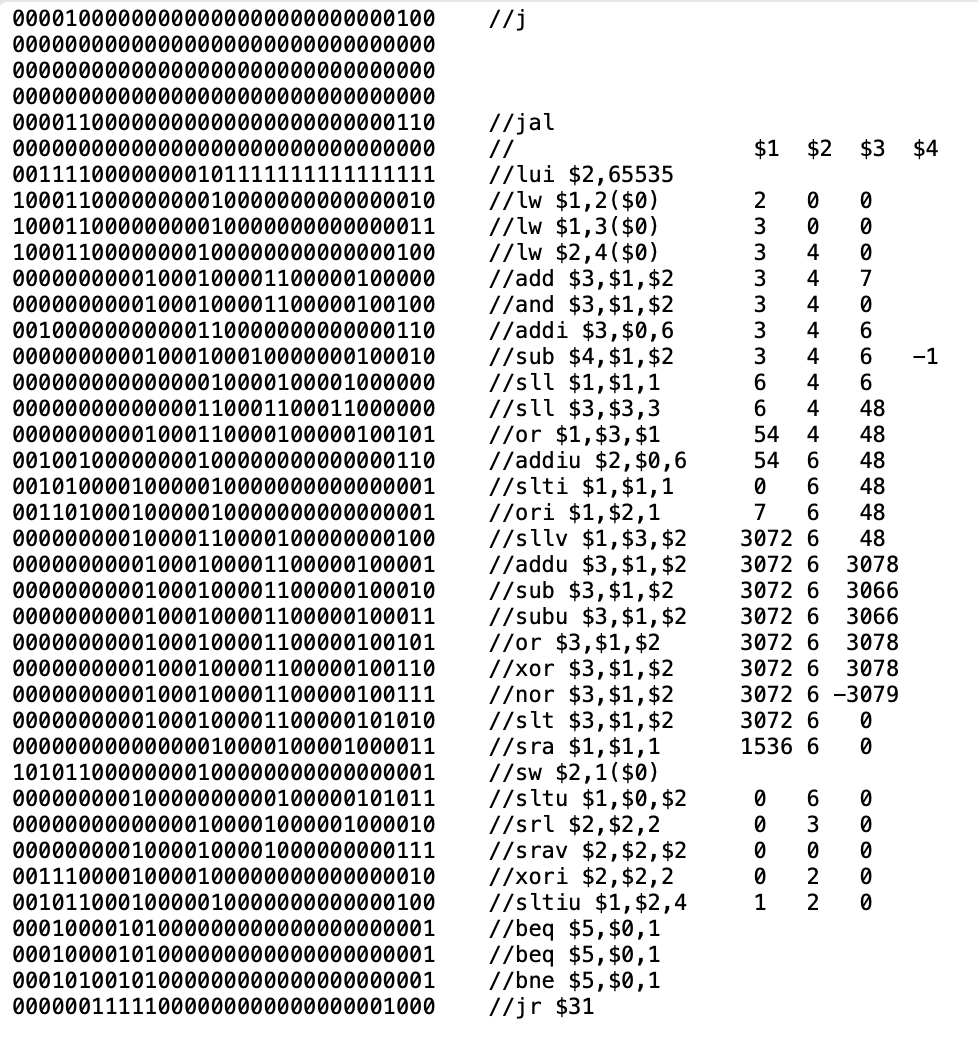
\includegraphics[width=0.6\textwidth]{./instruction.png}
    \caption{仿真测试指令集}
    \label{instruction}
\end{figure}

\begin{figure}[!h]
    \centering
    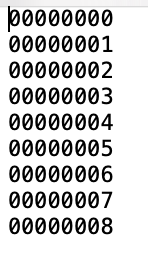
\includegraphics[width=0.3\textwidth]{./initialization.png}
    \caption{仿真测试数据集}
    \label{initialization}
\end{figure}

在编写激励代码的时候,依然使用了Verilog中的\texttt{\$readmemb}函数,这个函数可以将文件中的数据读入到指定的变量中。激励代码如下。

\begin{lstlisting}[language=Verilog]
module single_cycle_cpu_tb();

    reg clk;
    reg reset;

    Top top(
        .clk(clk),
        .reset(reset)
    );

    initial begin
        $readmemb("mem_inst.txt", top.inst_mem.instFile);
        $readmemb("mem_data.txt", top.memory.mem.memFile);
        reset = 1;
        clk = 0;
    end

    always #20 clk = ~clk;

    initial begin
        #30 reset = 0;
        #3000;
        $finish;
    end
endmodule
\end{lstlisting}

在运行仿真之后得到了如图\ref{result1},\ref{result2}所示的仿真结果。
\begin{figure}[!h]
    \centering
    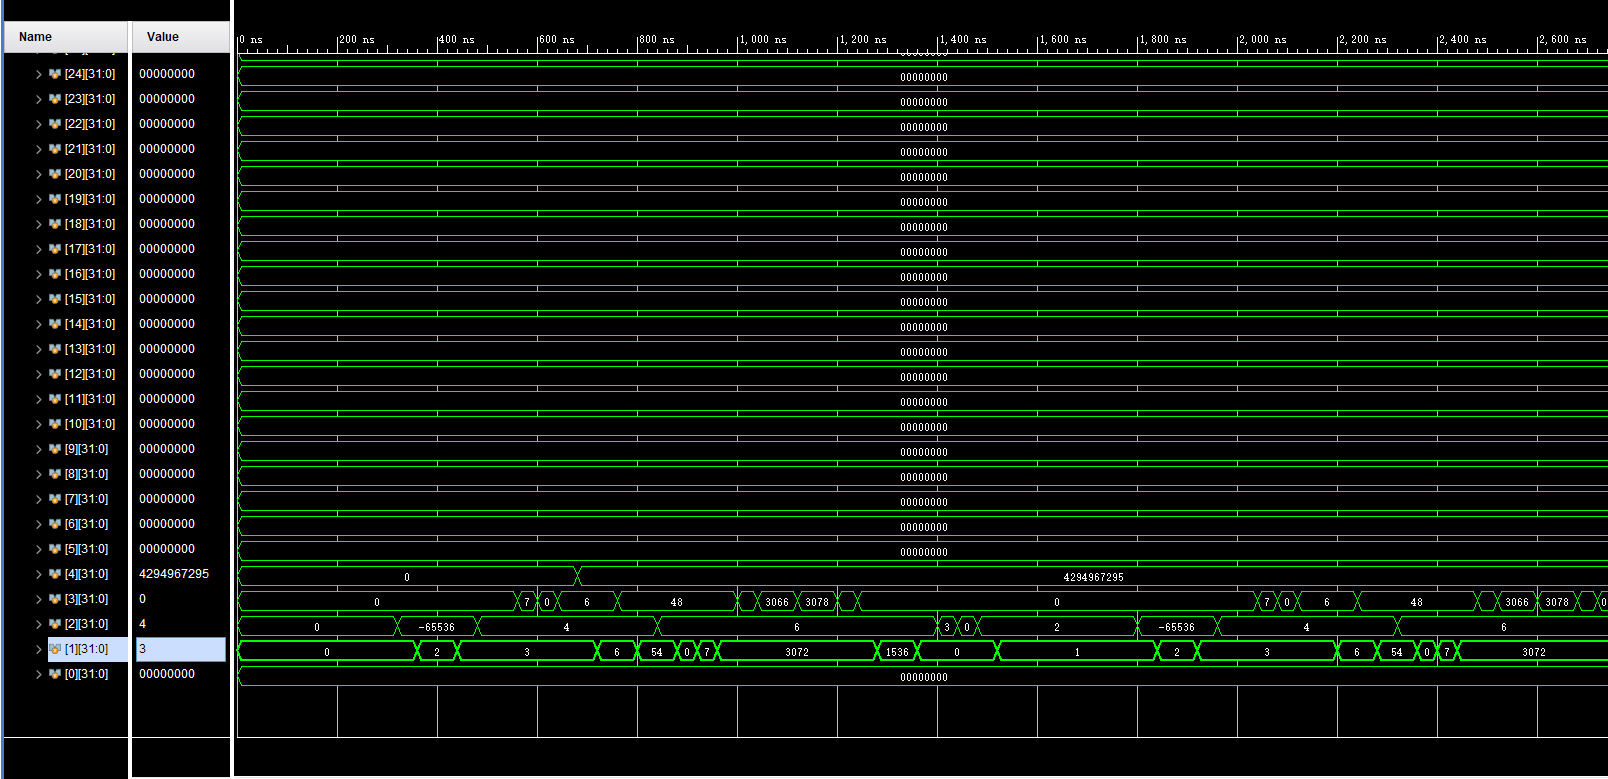
\includegraphics[width=0.8\textwidth]{./result1.png}
    \caption{仿真结果截图}
    \label{result1}
\end{figure}

\begin{figure}[!h]
    \centering
    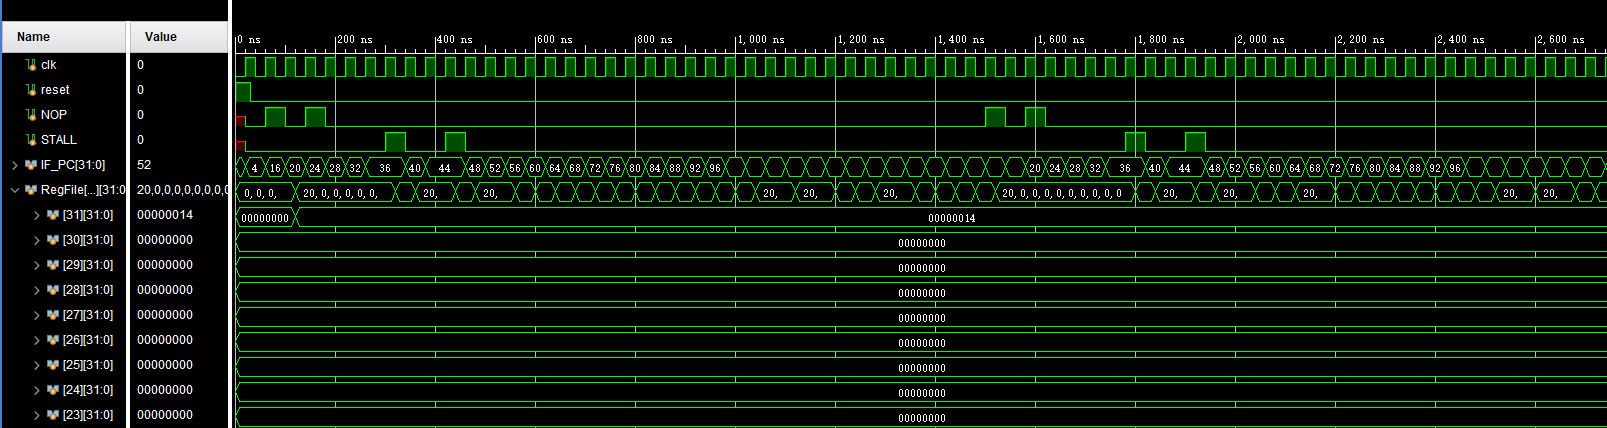
\includegraphics[width=0.8\textwidth]{./result2.png}
    \caption{仿真结果截图}
    \label{result2}
\end{figure}

可见结果符合预期,即当前实现的支持31条指令的简单多周期处理器的功能正确无误。

\section{总结与反思}
在本实验中,我学习并实现了前向传递(Forwarding)、停顿(Stall)、预测不转移(Predict-not-taken),了解了在实现流水线处理器的时候如何解决以跳转指令为典型的可能带来数据冒险、控制冒险和结构冒险,同时对处理器的效率进行优化。
除此以外,我还将本处理器支持的指令数由16条扩展成31条。主要的改动是增加了现有指令的无符号版本,这也充分利用了有符号扩展单元(Sign extension)会根据是否需要有符号扩展的性质,所以对整体的改动并不大,只需要修改主控制模块(Ctr)和
运算单元控制模块(ALUCtr)即可。

经过六次课的循序渐进的铺垫与练习,我最终实现了简单的多周期流水线处理器。此次实验让我充分的意识到了模块化开发的重要性,将一个大的模块划分成若干基本子模块,利用wire进行模块间的通信。最后利用顶层模块串联子模块,并且实现复杂的控制逻辑,如停顿、前向传递等。

除此以外,经过六次课的练习使我对硬件编程语言Verilog和软件Vivado有了较为深入的理解,在日后想进行相关方面的研究时会更加轻松的上手。这些收获让我获益匪浅。

\section{致谢}
感谢刘老师和数位助教老师的耐心指导与答疑;

感谢课程相关老师提供了详细的实验指导书来辅助同学更好地理解Verilog语言和Vivado软件;

感谢电子信息与电气工程学院提供了上机编程和上板验证的环境与条件。

再次感谢每一位老师和同学!